\documentclass[11pt,a4paper]{report}
\usepackage[textwidth=37em,vmargin=30mm]{geometry}
\usepackage{calc,xunicode,amsmath,amssymb,paralist,enumitem,tabu,booktabs,datetime2,xeCJK,xeCJKfntef,listings}
\usepackage{tocloft,fancyhdr,tcolorbox,xcolor,graphicx,eso-pic,xltxtra,xelatexemoji}

\newcommand{\envyear}[0]{2025}
\newcommand{\envdatestr}[0]{2025-03-01}
\newcommand{\envfinaldir}[0]{webdb/2025/20250301/final}

\usepackage[hidelinks]{hyperref}
\hypersetup{
    colorlinks=false,
    pdfpagemode=FullScreen,
    pdftitle={Web Digest - \envdatestr}
}

\setlength{\cftbeforechapskip}{10pt}
\renewcommand{\cftchapfont}{\rmfamily\bfseries\large\raggedright}
\setlength{\cftbeforesecskip}{2pt}
\renewcommand{\cftsecfont}{\sffamily\small\raggedright}

\setdefaultleftmargin{2em}{2em}{1em}{1em}{1em}{1em}

\usepackage{xeCJK,xeCJKfntef}
\xeCJKsetup{PunctStyle=plain,RubberPunctSkip=false,CJKglue=\strut\hskip 0pt plus 0.1em minus 0.05em,CJKecglue=\strut\hskip 0.22em plus 0.2em}
\XeTeXlinebreaklocale "zh"
\XeTeXlinebreakskip = 0pt


\setmainfont{Brygada 1918}
\setromanfont{Brygada 1918}
\setsansfont{IBM Plex Sans}
\setmonofont{JetBrains Mono NL}
\setCJKmainfont{Noto Serif CJK SC}
\setCJKromanfont{Noto Serif CJK SC}
\setCJKsansfont{Noto Sans CJK SC}
\setCJKmonofont{Noto Sans CJK SC}

\setlength{\parindent}{0pt}
\setlength{\parskip}{8pt}
\linespread{1.15}

\lstset{
	basicstyle=\ttfamily\footnotesize,
	numbersep=5pt,
	backgroundcolor=\color{black!5},
	showspaces=false,
	showstringspaces=false,
	showtabs=false,
	tabsize=2,
	captionpos=b,
	breaklines=true,
	breakatwhitespace=true,
	breakautoindent=true,
	linewidth=\textwidth
}






\newcommand{\coverpic}[2]{
    % argv: itemurl, authorname
    Cover photo by #2~~(\href{#1}{#1})
}
\newcommand{\makeheader}[0]{
    \begin{titlepage}
        % \newgeometry{hmargin=15mm,tmargin=21mm,bmargin=12mm}
        \begin{center}
            
            \rmfamily\scshape
            \fontspec{BaskervilleF}
            \fontspec{Old Standard}
            \fontsize{59pt}{70pt}\selectfont
            WEB\hfill DIGEST
            
            \vfill
            % \vskip 30pt
            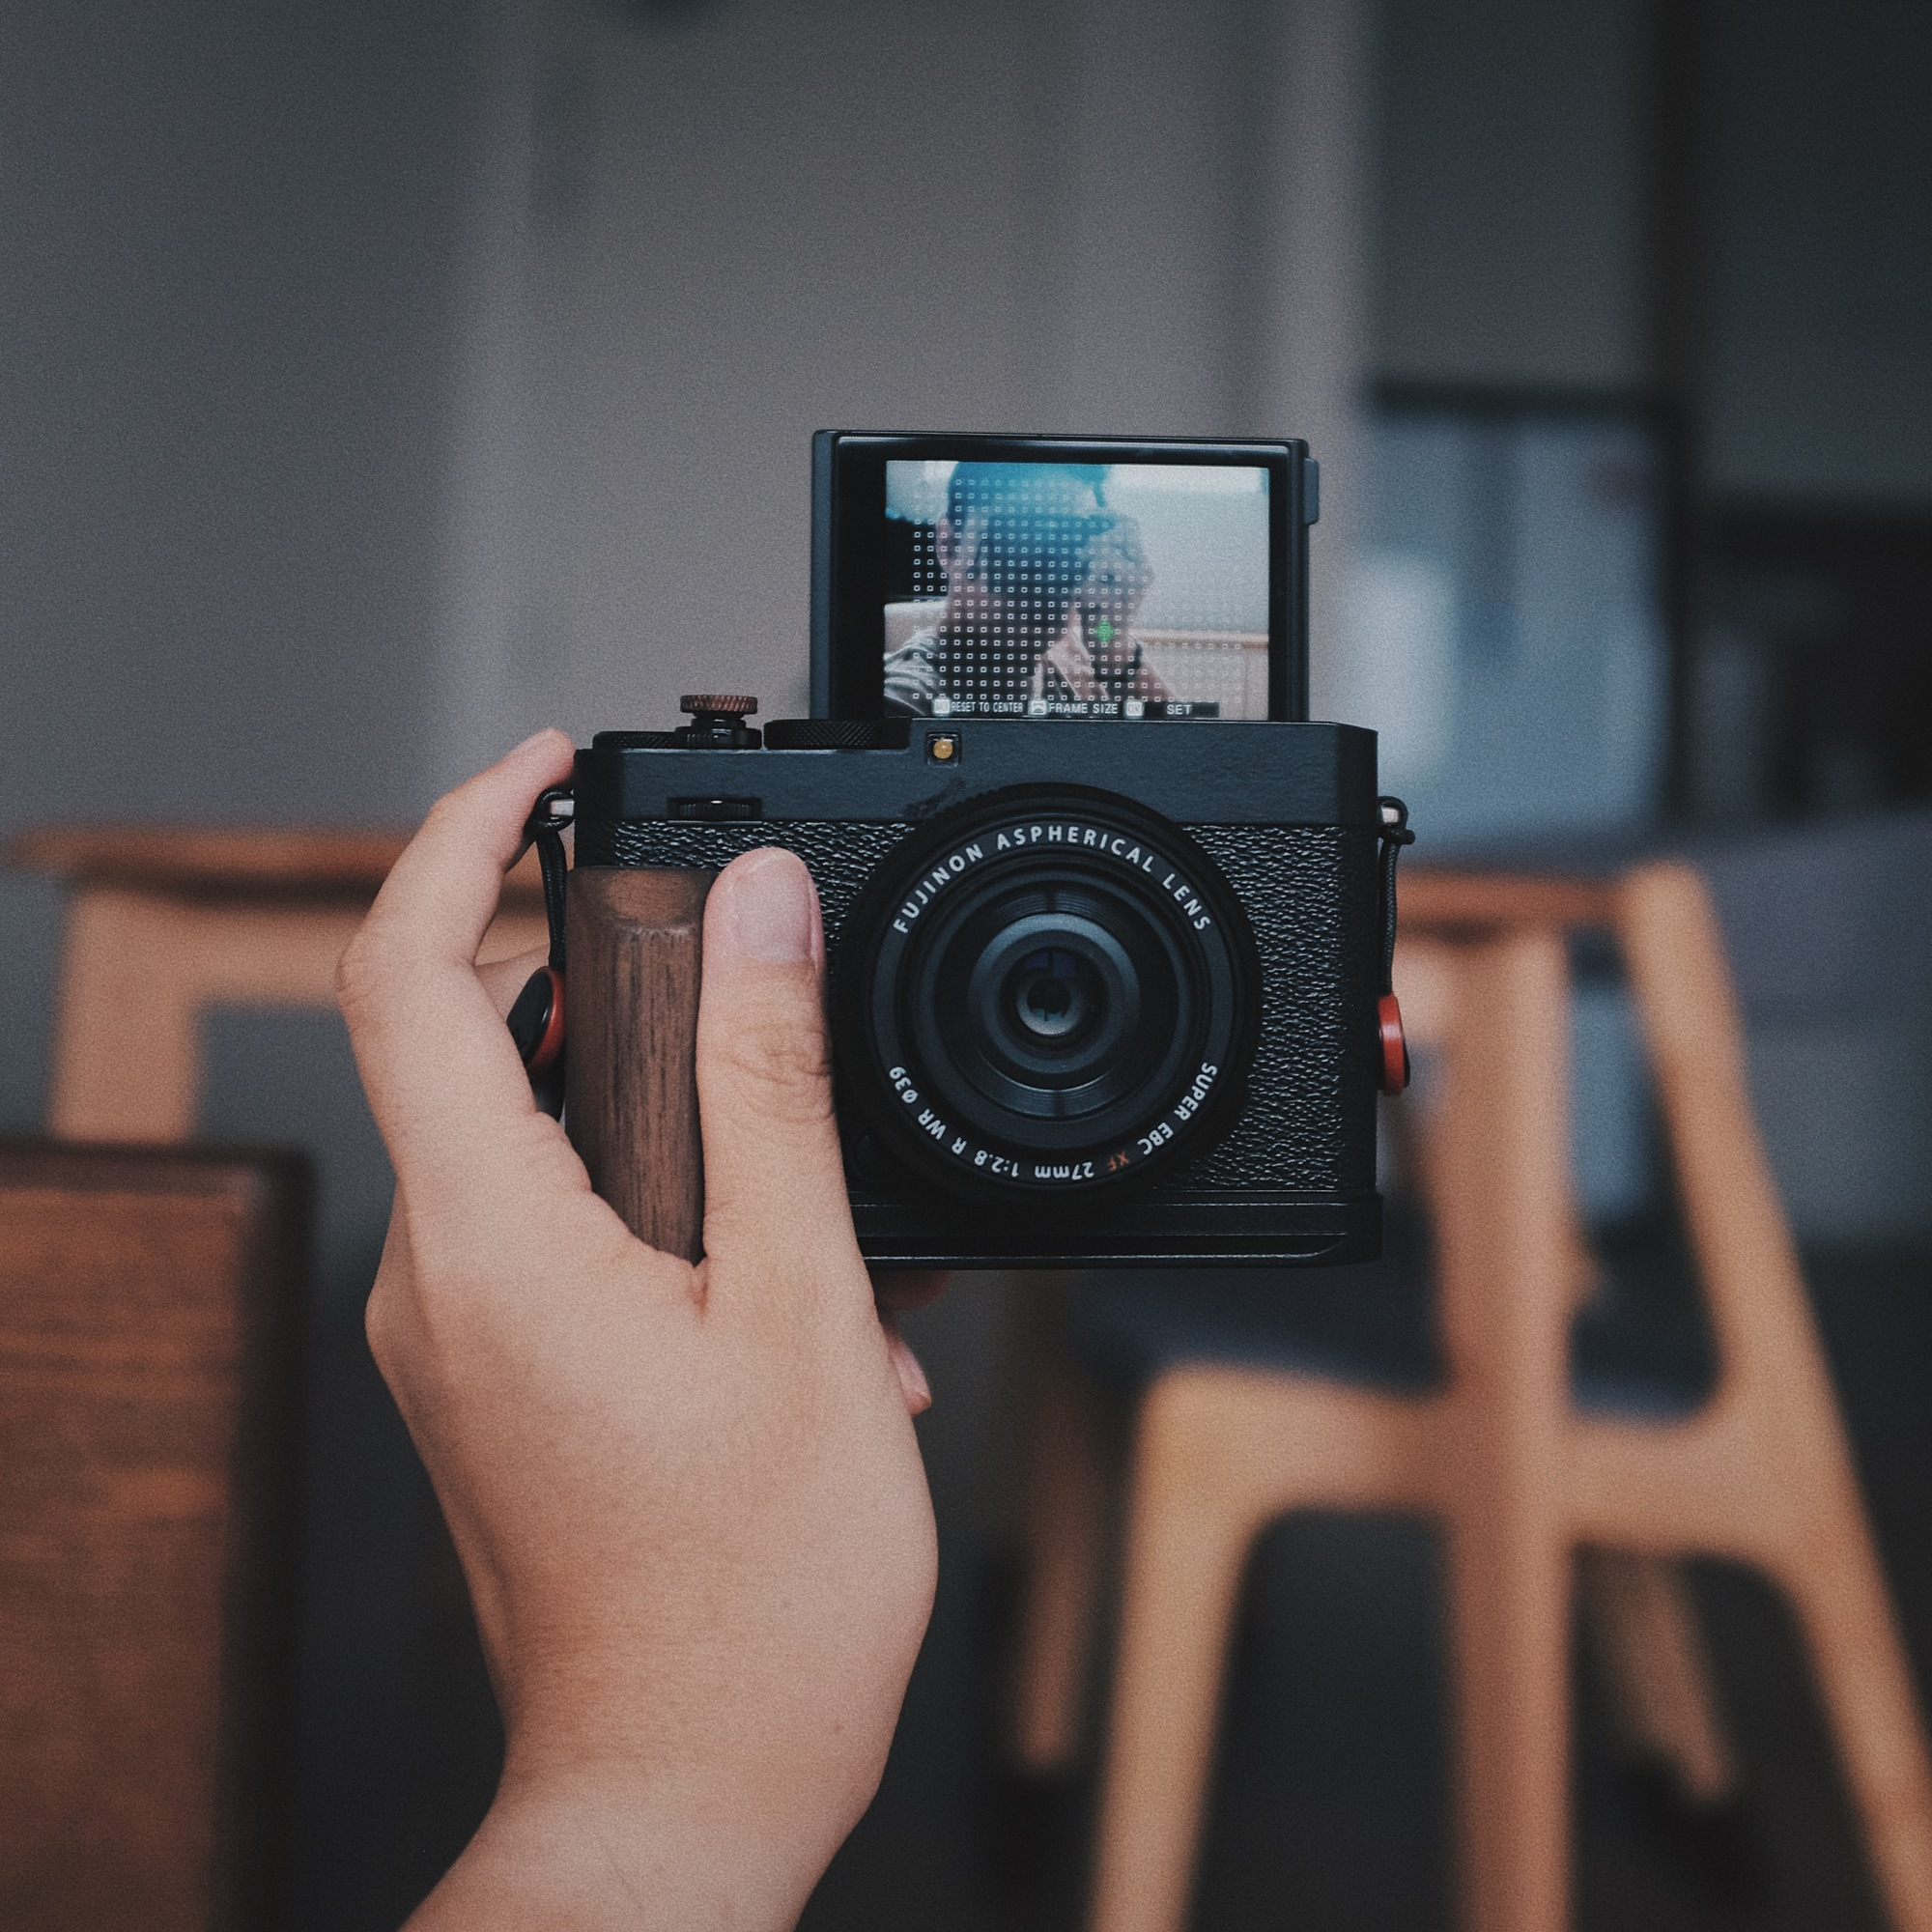
\includegraphics[width=\linewidth]{\envfinaldir/coverpic-prod.jpg}\par
            % \vskip 30pt
            \vfill

            \normalsize\rmfamily\scshape
            \copyright{} The Web Digest Project \hfill\large \envdatestr
        \end{center}
    \end{titlepage}
    % \restoregeometry
}
\newcommand{\simplehref}[1]{%
    \textcolor{blue!80!green}{\href{#1}{#1}}%
}
\renewcommand{\contentsname}{\center\Huge\sffamily\bfseries Contents\par\vskip 20pt}
\newcounter{ipartcounter}
\setcounter{ipartcounter}{0}
\newcommand{\ipart}[1]{
    % \vskip 20pt
    \clearpage
    \stepcounter{ipartcounter}
    \phantomsection
    \addcontentsline{toc}{chapter}{#1}
    % \begin{center}
    %     \Huge
    %     \sffamily\bfseries
    %     #1
    % \end{center}
    % \vskip 20pt plus 7pt
}
\newcounter{ichaptercounter}
\setcounter{ichaptercounter}{0}
\newcommand{\ichapter}[1]{
    % \vskip 20pt
    \clearpage
    \stepcounter{ichaptercounter}
    \phantomsection
    \addcontentsline{toc}{section}{\numberline{\arabic{ichaptercounter}}#1}
    \begin{center}
        \Huge
        \sffamily\bfseries
        #1
    \end{center}
    \vskip 20pt plus 7pt
}
\newcommand{\entrytitlefont}[1]{\subsection*{\raggedright\Large\sffamily\bfseries#1}}
\newcommand{\entryitemGeneric}[2]{
    % argv: title, url
    \parbox{\linewidth}{
        \entrytitlefont{#1}\par\vskip 5pt
        \footnotesize\ttfamily\mdseries
        \simplehref{#2}
    }\vskip 11pt plus 11pt minus 1pt
}
\newcommand{\entryitemGithub}[3]{
    % argv: title, url, desc
    \parbox{\linewidth}{
        \entrytitlefont{#1}\par\vskip 5pt
        \footnotesize\ttfamily\mdseries
        \simplehref{#2}\par\vskip 5pt
        \small\rmfamily\mdseries#3
    }\vskip 11pt plus 11pt minus 1pt
}
\newcommand{\entryitemAp}[3]{
    % argv: title, url, desc
    \parbox{\linewidth}{
        \entrytitlefont{#1}\par\vskip 5pt
        \footnotesize\ttfamily\mdseries
        \simplehref{#2}\par\vskip 5pt
        \small\rmfamily\mdseries#3
    }\vskip 11pt plus 11pt minus 1pt
}
\newcommand{\entryitemHackernews}[3]{
    % argv: title, hnurl, rawurl
    % \parbox{\linewidth}{
    %     \entrytitlefont{#1}\par\vskip 5pt
    %     \footnotesize\ttfamily\mdseries
    %     \simplehref{#3}\par
    %     \textcolor{black!50}{\href{#2}{#2}}
    % }\vskip 11pt plus 11pt minus 1pt
    \begin{minipage}{\linewidth}
            \entrytitlefont{#1}\par\vskip 5pt
            \footnotesize\ttfamily\mdseries
            \simplehref{#3}\par
            \textcolor{black!50}{\href{#2}{#2}}
    \end{minipage}\par\vskip 11pt plus 11pt minus 1pt
}







\begin{document}

\makeheader

\tableofcontents\clearpage




\ipart{Developers}
\ichapter{Hacker News}
\entryitemTwoLinks{Brian Krebs: This Administration Is Completely Compromised}{https://news.ycombinator.com/item?id=43211506}{https://infosec.exchange/@briankrebs/114083485241630234}

\entryitemTwoLinks{How to gain code execution on hundreds of millions of people and popular apps}{https://news.ycombinator.com/item?id=43210858}{https://kibty.town/blog/todesktop/}

\entryitemTwoLinks{Zelensky leaves White House after angry meeting}{https://news.ycombinator.com/item?id=43208973}{https://www.bbc.com/news/live/c625ex282zzt}

\entryitemTwoLinks{3,200\% CPU Utilization}{https://news.ycombinator.com/item?id=43207831}{https://josephmate.github.io/2025-02-26-3200p-cpu-util/}

\entryitemTwoLinks{Violence alters human genes for generations, researchers discover}{https://news.ycombinator.com/item?id=43206722}{https://news.ufl.edu/2025/02/syrian-violence-epigenetics/}

\entryitemTwoLinks{Write to Escape Your Default Setting}{https://news.ycombinator.com/item?id=43206174}{https://kupajo.com/write-to-escape-your-default-setting/}

\entryitemTwoLinks{May 5, Microsoft's Skype will shut down for good}{https://news.ycombinator.com/item?id=43205677}{https://arstechnica.com/gadgets/2025/02/on-may-5-microsofts-skype-will-shut-down-for-good/}

\entryitemTwoLinks{Starlink to take over \$2.4B contract to overhaul air traffic control comms}{https://news.ycombinator.com/item?id=43205435}{https://www.theverge.com/news/620777/starlink-verizon-contract-faa-communication-musk}

\entryitemTwoLinks{Waterfox: Fast and Private Web Browser}{https://news.ycombinator.com/item?id=43205110}{https://www.waterfox.net/}

\entryitemTwoLinks{Netboot Windows 11 with iSCSI and iPXE}{https://news.ycombinator.com/item?id=43204604}{https://terinstock.com/post/2025/02/Netboot-Windows-11-with-iSCSI-and-iPXE/}

\entryitemTwoLinks{WebShield – A new wide-spectrum content blocker for Safari}{https://news.ycombinator.com/item?id=43204406}{https://github.com/arjpar/WebShield}

\entryitemTwoLinks{A Comment on Mozilla's Policy Changes}{https://news.ycombinator.com/item?id=43204376}{https://www.waterfox.net/blog/a-comment-on-mozilla-changes/}

\entryitemTwoLinks{Github scam investigation: Thousands of ``mods'' and ``cracks'' stealing data}{https://news.ycombinator.com/item?id=43203158}{https://timsh.org/github-scam-investigation-thousands-of-mods-and-cracks-stealing-your-data/}

\entryitemTwoLinks{Mozilla deletes promise to never sell Firefox data}{https://news.ycombinator.com/item?id=43203096}{https://twitter.com/LundukeJournal/status/1895249805338886591}

\entryitemTwoLinks{Boris Spassky: 1937–2025}{https://news.ycombinator.com/item?id=43202982}{https://en.chessbase.com/post/boris-spassky-1937-2025}

\entryitemTwoLinks{WASM Wayland Web (WWW)}{https://news.ycombinator.com/item?id=43202773}{https://joeyh.name/blog/entry/WASM\_Wayland\_Web\_WWW/}

\entryitemTwoLinks{Microsoft is killing Skype}{https://news.ycombinator.com/item?id=43202052}{https://www.windowscentral.com/microsoft/microsoft-is-reportedly-killing-skype-after-14-years-of-neglect}

\entryitemTwoLinks{Microsoft begins turning off uBlock Origin and other extensions in Edge}{https://news.ycombinator.com/item?id=43201974}{https://www.neowin.net/news/microsoft-begins-turning-off-ublock-origin-and-other-extensions-in-edge/}

\entryitemTwoLinks{Mozilla introduces a Terms of Use agreement for Firefox}{https://news.ycombinator.com/item?id=43201869}{https://connect.mozilla.org/t5/discussions/information-about-the-new-terms-of-use-and-updated-privacy/m-p/87735\#M33600}

\entryitemTwoLinks{US authorities can see more than ever, with Big Tech as their eyes}{https://news.ycombinator.com/item?id=43201732}{https://proton.me/blog/big-tech-data-requests-surge}\ichapter{Phoronix}
\entryitemGeneric{\hskip 0pt{}NVIDIA Vulkan Beta Driver Updated For Blackwell \& New Extensions}{https://www.phoronix.com/news/NVIDIA-Vulkan-Beta-EO-Feb-2025}

\entryitemGeneric{\hskip 0pt{}AMD Prepares Linux Driver Support For Image Signal Processor With New Laptops}{https://www.phoronix.com/news/AMD-ISP4-Linux-Laptop-Driver}

\entryitemGeneric{\hskip 0pt{}FreeDesktop.org Devises New Hosting Plan For GitLab Infrastructure}{https://www.phoronix.com/news/FreeDesktop.org-Hosting-2025}

\entryitemGeneric{\hskip 0pt{}NetworkManager 1.52 Brings IPVLAN Interface Support, Ethtool FEC Mode}{https://www.phoronix.com/news/NetworkManager-1.52-Released}

\entryitemGeneric{\hskip 0pt{}AMD Radeon RX 9070 Series Officially Announced}{https://www.phoronix.com/review/amd-radeon-rx-9070-rdna4}

\entryitemGeneric{\hskip 0pt{}There Will Not Be Official ROCm Support For The Radeon RX 9070 Series On Launch Day}{https://www.phoronix.com/news/AMD-ROCm-RX-9070-Launch-Day}

\entryitemGeneric{\hskip 0pt{}AMD Engineer Talks Up Vulkan/SPIR-V As Part Of Their MLIR-Based Unified AI Software Play}{https://www.phoronix.com/news/AMD-Vulkan-SPIR-V-Wide-AI}

\entryitemGeneric{\hskip 0pt{}GCC 15.1 Compiler Nears Release As Bugs Whittled Away}{https://www.phoronix.com/news/GCC-15.1-Coming-Soon}

\entryitemGeneric{\hskip 0pt{}RADV Driver Expands Use Of Performance-Helping DCC Fast Clears On RDNA3 GPUs}{https://www.phoronix.com/news/RADV-DCC-More-RDNA3-Clears}\ichapter{Dribbble}
\entryitemGeneric{\hskip 0pt{}Letter A}{https://dribbble.com/shots/25691267-Letter-A}

\entryitemGeneric{\hskip 0pt{}Tally Logo Design}{https://dribbble.com/shots/25693309-Tally-Logo-Design}

\entryitemGeneric{\hskip 0pt{}Detective Dog Logo}{https://dribbble.com/shots/25692587-Detective-Dog-Logo}

\entryitemGeneric{\hskip 0pt{}HyperSeed - Logo Design}{https://dribbble.com/shots/25692269-HyperSeed-Logo-Design}

\entryitemGeneric{\hskip 0pt{}Logo Design for Gaming Platform (Unused for Sale)}{https://dribbble.com/shots/25692257-Logo-Design-for-Gaming-Platform-Unused-for-Sale}

\entryitemGeneric{\hskip 0pt{}Barbershop app dashboard}{https://dribbble.com/shots/25687859-Barbershop-app-dashboard}

\entryitemGeneric{\hskip 0pt{}Ramotion Logo Design}{https://dribbble.com/shots/25582478-Ramotion-Logo-Design}

\entryitemGeneric{\hskip 0pt{}Cimet Stationery}{https://dribbble.com/shots/25687823-Cimet-Stationery}

\entryitemGeneric{\hskip 0pt{}Check Mark App Icon}{https://dribbble.com/shots/25687869-Check-Mark-App-Icon}

\entryitemGeneric{\hskip 0pt{}Block13 Promo Board Design}{https://dribbble.com/shots/25688403-Block13-Promo-Board-Design}

\entryitemGeneric{\hskip 0pt{}Letter a}{https://dribbble.com/shots/25680095-Letter-a}

\entryitemGeneric{\hskip 0pt{}auren - logo design}{https://dribbble.com/shots/25681046-auren-logo-design}

\entryitemGeneric{\hskip 0pt{}Block13 Skateboards \& Sreetwear}{https://dribbble.com/shots/25683504-Block13-Skateboards-Sreetwear}

\entryitemGeneric{\hskip 0pt{}Quokka Mascot}{https://dribbble.com/shots/25681470-Quokka-Mascot}

\entryitemGeneric{\hskip 0pt{}Cardi C}{https://dribbble.com/shots/25678066-Cardi-C}

\entryitemGeneric{\hskip 0pt{}R}{https://dribbble.com/shots/25673587-R}

\entryitemGeneric{\hskip 0pt{}Fitme home landing page}{https://dribbble.com/shots/25674639-Fitme-home-landing-page}

\entryitemGeneric{\hskip 0pt{}Triceratops Dino}{https://dribbble.com/shots/25676249-Triceratops-Dino}

\entryitemGeneric{\hskip 0pt{}Illustrated Icons - American Home Shield}{https://dribbble.com/shots/25666386-Illustrated-Icons-American-Home-Shield}

\entryitemGeneric{\hskip 0pt{}Unused Geometric Fox}{https://dribbble.com/shots/25677006-Unused-Geometric-Fox}

\entryitemGeneric{\hskip 0pt{}Tiger Style}{https://dribbble.com/shots/25676567-Tiger-Style}

\entryitemGeneric{\hskip 0pt{}Logo Tip 002. Rhythm in Logo Design}{https://dribbble.com/shots/25674872-Logo-Tip-002-Rhythm-in-Logo-Design}

\entryitemGeneric{\hskip 0pt{}The Business}{https://dribbble.com/shots/25676385-The-Business}

\entryitemGeneric{\hskip 0pt{}Cute Dinosaur}{https://dribbble.com/shots/25671549-Cute-Dinosaur}


\ipart{Developers~~~~(zh-Hans)}
\ichapter{Solidot}
\entryitemGeneric{\hskip 0pt{}英国研究称散步有助于改善父女关系}{https://www.solidot.org/story?sid=80682}

\entryitemGeneric{\hskip 0pt{}暴力引发的基因表观遗传能持续数代}{https://www.solidot.org/story?sid=80681}

\entryitemGeneric{\hskip 0pt{}维苏威火山突然喷发致大脑组织玻璃化}{https://www.solidot.org/story?sid=80680}

\entryitemGeneric{\hskip 0pt{}过度种植抗根虫玉米会产生长期危害}{https://www.solidot.org/story?sid=80679}

\entryitemGeneric{\hskip 0pt{}日企计划 2027 年启动太空垃圾捕获试验}{https://www.solidot.org/story?sid=80678}

\entryitemGeneric{\hskip 0pt{}2024 年日本出生人数创历史最低}{https://www.solidot.org/story?sid=80677}

\entryitemGeneric{\hskip 0pt{}Microsoft Edge 准备淘汰 Manifest V2 扩展开始禁用 uBlock Origin}{https://www.solidot.org/story?sid=80676}

\entryitemGeneric{\hskip 0pt{}OpenAI 推出 GPT-4.5}{https://www.solidot.org/story?sid=80675}

\entryitemGeneric{\hskip 0pt{}Meta 解雇了约 20 名泄密的员工}{https://www.solidot.org/story?sid=80674}

\entryitemGeneric{\hskip 0pt{}EA 开源命令与征服系列游戏}{https://www.solidot.org/story?sid=80673}

\entryitemGeneric{\hskip 0pt{}Fish Shell 4.0 释出}{https://www.solidot.org/story?sid=80672}

\entryitemGeneric{\hskip 0pt{}激素疗法或有助于延缓皮肤衰老}{https://www.solidot.org/story?sid=80671}

\entryitemGeneric{\hskip 0pt{}Ocean Infinity 重新开始搜寻 MH370}{https://www.solidot.org/story?sid=80670}

\entryitemGeneric{\hskip 0pt{}暗能量光谱仪发现 2800 个候选黑洞}{https://www.solidot.org/story?sid=80669}

\entryitemGeneric{\hskip 0pt{}东京推行四天工作制试图平衡工作和生活}{https://www.solidot.org/story?sid=80668}

\entryitemGeneric{\hskip 0pt{}Firefox 公布使用条款和更新隐私条款}{https://www.solidot.org/story?sid=80667}

\entryitemGeneric{\hskip 0pt{}Automattic 可能面临集体诉讼}{https://www.solidot.org/story?sid=80666}

\entryitemGeneric{\hskip 0pt{}中国湿地总面积过去四十年净减少 6 万平方公里}{https://www.solidot.org/story?sid=80665}

\entryitemGeneric{\hskip 0pt{}极端高温可能进一步加速老年人衰老}{https://www.solidot.org/story?sid=80664}

\entryitemGeneric{\hskip 0pt{}新发现再次否定了佩托悖论}{https://www.solidot.org/story?sid=80663}\ichapter{V2EX}
\entryitemGeneric{\hskip 0pt{}[硬件] 寻找硬件合伙人,共同完成项目}{https://www.v2ex.com/t/1115022}

\entryitemGeneric{\hskip 0pt{}[问与答] 安卓苹果互传文件求推荐}{https://www.v2ex.com/t/1115021}

\entryitemGeneric{\hskip 0pt{}[职场话题] 最近几次 Technical Interview 的复盘}{https://www.v2ex.com/t/1115020}

\entryitemGeneric{\hskip 0pt{}[分享创造] 发现了个新词,连夜做了一个简单的网站,测试下收录速度~}{https://www.v2ex.com/t/1115019}

\entryitemGeneric{\hskip 0pt{}[问与答] 寻一个多时区时间展示工具}{https://www.v2ex.com/t/1115018}

\entryitemGeneric{\hskip 0pt{}[问与答] 小朋友学习机 App 上架平台在哪里?}{https://www.v2ex.com/t/1115016}

\entryitemGeneric{\hskip 0pt{}[程序员] vscer - VS Code 扩展离线下载命令行工具}{https://www.v2ex.com/t/1115014}

\entryitemGeneric{\hskip 0pt{}[酷工作] [南宁]找 Flutter 和 React (外地可远程) | 8-12K}{https://www.v2ex.com/t/1115011}

\entryitemGeneric{\hskip 0pt{}[问与答] 公司业务想上云,请推荐腾讯云的高级代理商}{https://www.v2ex.com/t/1115010}

\entryitemGeneric{\hskip 0pt{}[宽带症候群] 上海广电推大上行家宽}{https://www.v2ex.com/t/1115009}

\entryitemGeneric{\hskip 0pt{}[Android] 红米 K80 中国版在德国无法连 5G,求助大佬分析解决}{https://www.v2ex.com/t/1115008}

\entryitemGeneric{\hskip 0pt{}[问与答] 宿舍出现矛盾后解决的办法}{https://www.v2ex.com/t/1115005}

\entryitemGeneric{\hskip 0pt{}[投资] 最近实物黄金还能买吗?}{https://www.v2ex.com/t/1115004}

\entryitemGeneric{\hskip 0pt{}[分享发现] 新网站上线折腾半天才发现是 vercel 出现了生产故障}{https://www.v2ex.com/t/1115003}

\entryitemGeneric{\hskip 0pt{}[分享发现] 馒头站免,刷流吸血要抓紧了!}{https://www.v2ex.com/t/1115002}

\entryitemGeneric{\hskip 0pt{}[问与答] 有没有适配安卓平板的炒股(A 股)软件}{https://www.v2ex.com/t/1115001}

\entryitemGeneric{\hskip 0pt{}[推广] [AIBot 推广+送码] 功能超多、功能更新超激进的 AI 聚合平台,给我们一次机会,完整体验 AIBot 一次}{https://www.v2ex.com/t/1114999}

\entryitemGeneric{\hskip 0pt{}[问与答] 自建服务器有哪些好玩的脚本可以跑吗}{https://www.v2ex.com/t/1114995}

\entryitemGeneric{\hskip 0pt{}[OpenAI] 关于 claude 封号}{https://www.v2ex.com/t/1114994}

\entryitemGeneric{\hskip 0pt{}[健康] 百度热搜 22 岁女孩患罕见病全身似烧伤}{https://www.v2ex.com/t/1114992}

\entryitemGeneric{\hskip 0pt{}[分享发现] 飞书到底在干嘛?疯狂下载?}{https://www.v2ex.com/t/1114991}

\entryitemGeneric{\hskip 0pt{}[游戏] Avowed Game}{https://www.v2ex.com/t/1114990}

\entryitemGeneric{\hskip 0pt{}[程序员] 关于 cursor、windsurf 相关 ai 编辑器与工作流}{https://www.v2ex.com/t/1114989}

\entryitemGeneric{\hskip 0pt{}[生活] 今天哭的特别伤心}{https://www.v2ex.com/t/1114988}

\entryitemGeneric{\hskip 0pt{}[职场话题] 没有技术的外行大龄菜鸟想转行报班进入 IT 可行吗?}{https://www.v2ex.com/t/1114987}

\entryitemGeneric{\hskip 0pt{}[酷工作] [上海] 米哈游 miHoYo 2025.2.28 最新招聘信息}{https://www.v2ex.com/t/1114984}

\entryitemGeneric{\hskip 0pt{}[云计算] 备案域名使用 cloudflare 会有什么风险吗?}{https://www.v2ex.com/t/1114983}

\entryitemGeneric{\hskip 0pt{}[宽带症候群] 广州移动未开通 IPTV 业务可以使用吗}{https://www.v2ex.com/t/1114982}

\entryitemGeneric{\hskip 0pt{}[分享创造] 刚入手了一个域名 funny-coloring-pages.online 已上站}{https://www.v2ex.com/t/1114981}

\entryitemGeneric{\hskip 0pt{}[商业模式] 种田游戏的天花板,背后的程序员年入 3 亿美金}{https://www.v2ex.com/t/1114980}

\entryitemGeneric{\hskip 0pt{}[求职] 广东境内有好的外企推荐吗}{https://www.v2ex.com/t/1114979}

\entryitemGeneric{\hskip 0pt{}[程序员] 有项目源码的也可以 像他这样去卖, 单价 268 不便宜呢.}{https://www.v2ex.com/t/1114977}

\entryitemGeneric{\hskip 0pt{}[旅行] 简单记一次 9 天的日本桥(东京)到日本桥(大阪)单人骑游}{https://www.v2ex.com/t/1114976}

\entryitemGeneric{\hskip 0pt{}[酷工作] [缺人] 社招内推|拼多多集团-PDD|上海}{https://www.v2ex.com/t/1114975}

\entryitemGeneric{\hskip 0pt{}[Windows] Windows 11 出于什么理由把任务栏固定在屏幕底部?是技术原因吗?我从 Windows 95 开始就习惯把任务栏放屏幕顶上,切换程序很方便, Windows 11 连这个功能都砍}{https://www.v2ex.com/t/1114974}

\entryitemGeneric{\hskip 0pt{}[Flutter] 有没有可以学习的 flutter riverpod 的实战项目,希望推荐下更好的状态管理方案}{https://www.v2ex.com/t/1114973}

\entryitemGeneric{\hskip 0pt{}[问与答] 老哥们, 求一个开源 餐饮小程序 源码+后台}{https://www.v2ex.com/t/1114972}

\entryitemGeneric{\hskip 0pt{}[Twitter] 注册新账号把生日设定成注册当天,注册成功秒封禁}{https://www.v2ex.com/t/1114970}

\entryitemGeneric{\hskip 0pt{}[问与答] 通过 graphrag 生成了知识图谱 ,问下这个图谱哪种格式 可能结合 deepseek api 使用}{https://www.v2ex.com/t/1114969}

\entryitemGeneric{\hskip 0pt{}[生活] 5202 年,各位钱包里还会保留多少『实体钱』?}{https://www.v2ex.com/t/1114967}

\entryitemGeneric{\hskip 0pt{}[程序员] 有人会 textual 这个库的吗?我想修改 option\_list 里面的 option 高度和字体大小怎么弄啊?求指点.}{https://www.v2ex.com/t/1114966}

\entryitemGeneric{\hskip 0pt{}[Go 编程语言] 各位大佬们怎么进行 golang 项目的多版本控制?}{https://www.v2ex.com/t/1114965}

\entryitemGeneric{\hskip 0pt{}[Android] 现在,过 root 检测有什么比较好的方案吗?}{https://www.v2ex.com/t/1114964}

\entryitemGeneric{\hskip 0pt{}[Apple] Mac mini M4 搭配红米 A27U 显示器求助🙏}{https://www.v2ex.com/t/1114963}

\entryitemGeneric{\hskip 0pt{}[程序员] 为什么现在 AI 场景落地专门盯着代码辅助干?}{https://www.v2ex.com/t/1114962}

\entryitemGeneric{\hskip 0pt{}[Visual Studio Code] vscode 开发前端 js,有哪些扩展推荐?}{https://www.v2ex.com/t/1114960}

\entryitemGeneric{\hskip 0pt{}[分享创造] 我做了一个随机生成的工具合集站点,欢迎来玩。}{https://www.v2ex.com/t/1114959}

\entryitemGeneric{\hskip 0pt{}[Local LLM] Thinkstation P8 搭配 4090 48G 测试 Deepseek-r1}{https://www.v2ex.com/t/1114957}

\entryitemGeneric{\hskip 0pt{}[分享发现] cursor 速度飞升了,缓存了提问和回答??}{https://www.v2ex.com/t/1114956}

\entryitemGeneric{\hskip 0pt{}[Web Dev] 求推荐开源的工业领域电商项目}{https://www.v2ex.com/t/1114955}


\ipart{Generic News}
\ichapter{AP News}
\entryitemWithDescription{\hskip 0pt{}Rio's Carnival kicks off as mayor gives key to the city to King Momo}{https://apnews.com/article/49b8d45ace7262f956f2422aa8944c9d}{}

\entryitemWithDescription{\hskip 0pt{}A stretch of a North Carolina highway that collapsed during Helene is about to reopen}{https://apnews.com/article/85c84c5492d3d86d127cefcf77e23938}{}

\entryitemWithDescription{\hskip 0pt{}Microsoft shutting down Skype in May}{https://apnews.com/article/7ac4e86f55acb40098476e01d8d4a473}{}

\entryitemWithDescription{\hskip 0pt{}At least 25 workers are trapped by an avalanche in northern India}{https://apnews.com/article/6aff6772cdd48451ee450679dc621343}{}

\entryitemWithDescription{\hskip 0pt{}South Korean police summon Japanese woman for kissing BTS member without consent}{https://apnews.com/article/84e365169dff67e8758c440bf00bbb61}{}

\entryitemWithDescription{\hskip 0pt{}No new bombshells in Justice Department's release of Jeffrey Epstein files}{https://apnews.com/article/1a6af3e9fa1cfb6d267985a971a4929a}{}

\entryitemWithDescription{\hskip 0pt{}`Chicken Shop Date' creator Amelia Dimoldenberg brings flirty awkwardness to the Oscars red carpet}{https://apnews.com/article/79d9d4d6730dea4e7425b3f3eafbda2a}{}

\entryitemWithDescription{\hskip 0pt{}US porn actor visits Afghanistan in a trip unacknowledged by the Taliban}{https://apnews.com/article/abaa693d11e6af4c28a8509f80da1c18}{}

\entryitemWithDescription{\hskip 0pt{}Sarah Michelle Gellar, Taylor Momsen and Blake Lively mourn death of Michelle Trachtenberg}{https://apnews.com/article/c98de34f0c6feaa2b89d8f0c506a0ed5}{}

\entryitemWithDescription{\hskip 0pt{}Boris Spassky, Soviet chess champion who lost famed Cold War-era match to Bobby Fischer, dies at 88}{https://apnews.com/article/3ce0362af1ff27ea8c408237eabab1e3}{}

\entryitemWithDescription{\hskip 0pt{}Woman suspected in Colorado Tesla dealership vandalism charged in federal court}{https://apnews.com/article/d6aefe246624592ceff0b4e6ce6e57a1}{}

\entryitemWithDescription{\hskip 0pt{}A Florida Gator took on a Florida gator. Billy Horschel prevailed in the matchup at PGA National}{https://apnews.com/article/0b258d19581353bf0eac9081443c9e49}{}

\entryitemWithDescription{\hskip 0pt{}Pending US home sales slide to all-time low in January on rates, prices, maybe weather}{https://apnews.com/article/627425ea38f88c9e766d3c22e93a0f57}{}\ichapter{Reuters}
\entryitemWithDescription{\hskip 0pt{}Italy calls for summit between U.S. and Europeans, says divisions make West weaker}{https://www.reuters.com/world/italy-calls-summit-between-us-europeans-says-divisions-make-west-weaker-2025-02-28/}{Italy\textquotesingle s Prime Minister Giorgia Meloni on Friday said Italy would propose to its partners an immediate summit involving the United States and European nations and allies to discuss how "to deal with the great challenges of...}

\entryitemWithDescription{\hskip 0pt{}North Korea says senior official met Russian president Putin, KCNA says}{https://www.reuters.com/world/north-korea-says-senior-official-met-russian-president-putin-kcna-says-2025-02-28/}{Russian President Vladimir Putin held a meeting with a North Korean senior official in Moscow on Thursday, North Korea\textquotesingle s state news agency said on...}

\entryitemWithDescription{\hskip 0pt{}Russian air defences down 17 drones in six Russian regions}{https://www.reuters.com/world/europe/russian-air-defences-down-17-drones-six-russian-regions-2025-02-28/}{Russian air defences downed 17 drones in six Russian regions over a period of nearly 2-1/2 hours late on Friday, the Russian Defence Ministry...}

\entryitemWithDescription{\hskip 0pt{}Switzerland to host conference on occupied Palestinian territories on March 7}{https://www.reuters.com/world/middle-east/switzerland-host-conference-occupied-palestinian-territories-march-7-2025-02-28/}{Switzerland has invited 196 states who are parties to the Geneva Conventions to participate in a conference next week on the situation of civilians living in the Israeli occupied territories, a Foreign Ministry spokesperson said on...}

\entryitemWithDescription{\hskip 0pt{}Lawmakers in US Congress react to Zelenskiy-Trump Oval Office clash}{https://www.reuters.com/world/lawmakers-us-congress-react-zelenskiy-trump-oval-office-clash-2025-02-28/}{Ukrainian President Volodymyr Zelenskiy and U.S. President Donald Trumptraded blows at a White House meeting that ended in disaster on Friday, prompting an outpouring of reaction from members of Congress and other American public...}

\entryitemWithDescription{\hskip 0pt{}Mexico 'fast-track' expulsion of drug lords to US broke legal procedures, experts say}{https://www.reuters.com/world/americas/mexico-fast-track-expulsion-drug-lords-us-broke-legal-procedures-experts-say-2025-02-28/}{The Mexican government broke with its own legal procedures to hand over 29 suspected cartel members to the U.S., experts said, as pressure mounts over threats by President Donald Trump to slap tariffs on Mexican...}

\entryitemWithDescription{\hskip 0pt{}Brazil's finance minister isolated as market fears of a leftist pivot mount}{https://www.reuters.com/world/americas/brazils-finance-minister-isolated-market-fears-leftist-pivot-mount-2025-02-28/}{Brazil\textquotesingle s latest cabinet shuffle has left Finance Minister Fernando Haddad with no strong supporters in President Luiz Inacio Lula da Silva\textquotesingle s inner circle for his moderate fiscal approach, fueling fears of a...}

\entryitemWithDescription{\hskip 0pt{}Russians gloat over Zelenskiy's 'suicide in the White House'}{https://www.reuters.com/world/russian-security-official-medvedev-says-zelenskiy-got-solid-slap-white-house-2025-02-28/}{Russia reacted with glee on Friday to the bitter clash between Donald Trump and Volodymyr Zelenskiy in the White House, saying the Ukrainian leader got what he...}

\entryitemWithDescription{\hskip 0pt{}World reacts to Zelenskiy-Trump Oval Office clash}{https://www.reuters.com/world/world-reacts-zelenskiy-trump-oval-office-clash-2025-02-28/}{Ukrainian President Volodymyr Zelenskiy and U.S. President Donald Trumpclashed at a White House meeting that ended in disaster on Friday, prompting an outpouring of reaction from across the...}

\entryitemWithDescription{\hskip 0pt{}Zelenskiy, Trump clash will accelerate US probe of fraud in Ukraine aide, senior official says}{https://www.reuters.com/world/zelenskiy-trump-clash-will-accelerate-us-probe-fraud-ukraine-aide-senior-2025-02-28/}{Friday\textquotesingle s clash in the Oval Office between Ukrainian Prime Minister Volodymyr Zelenskiy and President Donald Trump will speed up Washington\textquotesingle s efforts to investigate any waste, fraud and abuse involving U.S...}

\entryitemWithDescription{\hskip 0pt{}Lebanon will ask Saudi Arabia to resume \$3-billion grant to army, president says}{https://www.reuters.com/world/middle-east/lebanon-will-ask-saudi-arabia-resume-3-billion-grant-army-president-says-2025-02-28/}{Lebanon\textquotesingle s President Joseph Aoun will ask Saudi Arabia to reactivate a \$3-billion aid package to the Lebanese army in his visit to the kingdom next week, Aoun said in an interview with Asharq television broadcast on...}

\entryitemWithDescription{\hskip 0pt{}Top Mexican prosecutor defends transfer of accused drug lords as legal}{https://www.reuters.com/world/americas/top-mexican-prosecutor-defends-transfer-accused-drug-lords-legal-2025-02-28/}{Mexican Attorney General Alejandro Gertz defended on Friday the legality of the government\textquotesingle s handover of 29 suspected cartel leaders to the United States a day earlier, arguing that national security laws allowed...}

\entryitemWithDescription{\hskip 0pt{}Trump, Zelenskiy did not sign minerals deal, White House says}{https://www.reuters.com/world/trump-zelenskiy-did-not-sign-minerals-deal-white-house-says-2025-02-28/}{U.S. President Donald Trump and Ukrainian President Volodymyr Zelenskiy did not sign a minerals deal on Friday, a White House official told...}\ichapter{联合早报}
\entryitemWithDescription{沈泽玮:台湾冲突阻遏法案只叫不咬?}{https://www.zaobao.com/news/china/story20240918-4758889}{美国众议院9月9日开启了长达一星期的``中国周'',共通过25项主要涉华法案。(法新社) 美国众议院在当地时间9月9日开启了长达一星期的``中国周'',在美国总统和国会选举举行之前,密集表决数十项与中国有关的法案,共通过25项主要涉华法案……}

\entryitemWithDescription{欧盟电动车关税投票倒计时 中国在分歧中寻支持}{https://www.zaobao.com/news/china/story20240917-4758953}{欧盟27个成员国将于9月25日就是否继续对进口自中国的电动汽车额外征税进行最后表决。图为上海港等待装运出口的电动汽车。(彭博社) 欧盟对中国电动汽车加征关税的投票进入倒计时,正在欧洲访问的中国商务部部长王文涛与欧盟多国政府高层就此进行协商,试图在立场分歧的成员国中争取到更多支持。 受访学者研判,欧盟对中国电动汽车加征关税不可避免,但具体的加税方式和幅度仍有一定弹性,这是王文涛此行与各国谈判的重点……}

\entryitemWithDescription{港府今年将举办逾400项国庆活动}{https://www.zaobao.com/news/china/story20240917-4759341}{再过十多天就是中国国庆75周年,香港天星小轮展示``国庆75周年''\,``三天免费搭小轮''等标语迎国庆。(中新社) 再过十多天就是中国国庆75周年,香港特区政府今年将举办逾400项庆祝活动,希望通过一连串活动庆祝国庆,并且弘扬爱国主义教育及刺激消费。 港府星期二(9月17日)召开记者会,介绍各项庆祝国庆活动和特别优惠,涉及出行及吃喝玩乐等领域……}

\entryitemWithDescription{美空军部长:中国大陆军演精密化 为入侵封锁台湾做准备}{https://www.zaobao.com/news/china/story20240917-4759407}{美国空军部长肯德尔星期一(9月16日)在空军暨太空军协会的一场大会上致辞,提到中国对印太地区日益增长的威胁。(取自美国国防部网站) (华盛顿综合讯)美国空军部长肯德尔指,中国大陆军演的规模越来越大,也更加精密化,这是在专门为入侵、封锁台湾做准备。他也称,中国对印太地区的威胁现在已存在……}

\entryitemWithDescription{批准潜在对台备件军售案后 美派巡逻机过航台海}{https://www.zaobao.com/news/china/story20240917-4758770}{台军士兵8月26日在屏东县枋山训练场进行实弹演习时,从M1167 TOW运载车上发射一枚美制TOW-2A线导反坦克导弹。(路透社) (华盛顿/台北/北京综合讯)在批准潜在对台备件军售案之后,美国派遣反潜巡逻机过航台湾海峡,中国人民解放军东部战区则组织战机跟监美机,并誓言``坚决捍卫国家主权''……}

\entryitemWithDescription{李家超:若香港驻美经贸办被关 受害的是美企}{https://www.zaobao.com/news/china/story20240917-4758797}{香港特首李家超星期一(9月17日)警告,如果美国通过法案,导致香港驻美经贸办关闭,受害的是美国企业。图为李家超9月11日在``一带一路''高峰论坛上致辞。(彭博社) (香港综合讯)香港特首李家超警告,如果美国通过法案,导致香港驻美经贸办关闭,受害的是美国企业。 美国众议院上周通过《香港经济贸易办事处认证法案》,如果参议院也表决通过并交由总统签署成法,香港三个驻美国的经贸办可能将被强制关闭……}

\entryitemWithDescription{美国指中国航空工业集团员工企图实施黑客攻击}{https://www.zaobao.com/news/china/story20240917-4757988}{(华盛顿综合讯)中国航空航天巨头中国航空工业集团一名员工被指试图对美国宇航局、美国军方和其他目标展开黑客攻击。 据彭博社报道,美国检察官布坎南星期一(9月16日)在起诉书中,指控中国航空工业集团39岁的工程师吴宋(音译,Song Wu)企图从美国宇航局、空军、陆军和海军,以及联邦航空管理局取得电脑软件和源代码……}

\entryitemWithDescription{【东谈西论】恒大账务造假 普华永道是共犯还是被拖累?}{https://www.zaobao.com/news/china/story20240917-4756452}{因涉及恒大地产审计项目的违法行为,普华永道中国9月13日被中国财政部和证监会处以4.41亿人民币罚款并被令停业六个月, 广州分所被撤销……}

\entryitemWithDescription{戴庆成:香港输入人才计划大检阅}{https://www.zaobao.com/news/china/story20240917-4744978}{香港于2022年底推出高端人才通行证计划。(法新社) 2019年香港反修例风波过后,数以十万计港人移居海外,令香港出现人才荒。港府为了解决这个问题,在过去几年积极引入``新血'',当中以高才通计划最受瞩目,社会上也不时热议其成效。 高才通全称为高端人才通行证计划,于2022年底推出,申请人年收入须达到250万港元(约42万新元)以上,或本科毕业于全球百强大学并满足一定工作年限等……}

\entryitemWithDescription{中美希望稳定双边关系 中小国家可​​​搭建桥梁}{https://www.zaobao.com/news/china/story20240917-4745091}{中美元首去年11月在旧金山会晤后,双方都希望稳定两国关系,我国巡回大使陈庆珠认为,如果中美两国都认为走向战争不符合它们的利益,那么中小国家就可以做点什么,为双方搭建桥梁。 陈庆珠星期一(9月16日)在李光耀公共政策学院的一场研讨会上说,中国与西方的关系面对诸多困难,有中国智库表示,希望新加坡能协助在中美之间建立更多对话,``因为新加坡受美国信任,也在中国有渠道''……}

\entryitemWithDescription{陈庆珠:世界经历了三次``中国冲击'' 中美的主导力之争将继续}{https://www.zaobao.com/news/china/story20240917-4744996}{李光耀公共政策学院``思想之节庆''的一场研讨会,讨论``历史终结时的中国冲击''。左起是我国巡回大使陈庆珠、通商中国主席李奕贤、李光耀公共政策学院国际关系助理教授何莉菁、李光耀公共政策学院院长柯成兴……}

\entryitemWithDescription{上海遭遇75年来最强台风 扰乱民众中秋假期出行}{https://www.zaobao.com/news/china/story20240916-4745224}{台风贝碧嘉星期一(9月16日)登陆上海,维护人员星期一下午在衡山路上处理倒伏的树木。 (新华社) 台风造成上海上万株数目倒伏或折断。图为一棵倒下的大树砸坏一旁的建筑。(法新社) 台风贝碧嘉登陆上海后,黄浦江苏州河口潮位上涨,乌云密布。(中新社) 中国上海市星期一(9月16日)遭遇75年来最强台风``贝碧嘉''登陆,也是上海有记录以来首次有强台风侵袭……}

\entryitemWithDescription{陆男频长驱偷渡台湾在测试边防实力?}{https://www.zaobao.com/news/china/story20240916-4745161}{中国大陆一名王姓男子在中秋节前夕,乘橡皮艇从浙江宁波抵达台湾新北市林口,主动打电话投案,海巡署人员前去接他上岸。(自由時報) 中国大陆一名王姓男子划橡皮艇于上星期六清晨偷渡到台湾,隔天被新北市地方法院裁定羁押禁见。这是6月以来第二起大陆人士偷渡至台湾,此间专家质疑是否为海防破口,并怀疑对岸是否在测试台湾的边防实力……}

\entryitemWithDescription{中美时隔八月举行国防部工作会晤}{https://www.zaobao.com/news/china/story20240916-4745025}{(北京/华盛顿综合讯)中美双方上周末举行国防部工作会晤;美国官员称,美国积极进行美中两军外交活动,不代表美国对有关中国议题的处理方式发生任何改变。 据中国国防部星期天(15日)晚上通报,北京香山论坛结束后,第18次中美国防部工作会晤上星期六至星期天(9月14日至15日)在北京举行……}

\entryitemWithDescription{中国高校今年拟增足球运动本科专业}{https://www.zaobao.com/news/china/story20240916-4744925}{(北京综合讯)为了培养足球专业人才,中国大专学府今年度拟新增足球运动本科专业,以具体落实中国足球改革。 综合人民网和《南方都市报》报道,中国教育部上星期五(9月13日)发布《2024年度普通高等学校本科专业申报材料公示》。根据公示统计,今年度拟新增专业535个,涉及353所高校,其中39所高校新增足球运动专业……}

\entryitemWithDescription{香港23条首案 港男因穿``光时''上衣被定罪}{https://www.zaobao.com/news/china/story20240916-4743439}{(香港综合讯)香港一名无业男子,今年6月因穿印有2019年反修例抗争口号的上衣而被捕。他星期一承认违反煽动意图罪,成为在《维护国家安全条例》(即《香港基本法》第23条)下被定罪的第一人。 综合港媒《星岛日报》和路透社报道,27岁无业男子诸启邦今年6月12日在石门港铁站附近,未能出示身份证供查阅被警方拘捕……}

\entryitemWithDescription{美国务院:中国释放被关押近20年美籍牧师}{https://www.zaobao.com/news/china/story20240916-4744614}{(华盛顿综合电)中国释放被关押近20年的美国籍牧师,显示北京在中美关系的关键时刻展现善意。 综合彭博社、法新社和路透社报道,美国国务院发言人星期天(9月15日)说:``我们欢迎林大卫(音译,David Lin)从中华人民共和国的监狱获释。他已回返美国,这是他近20年来首次与家人见面。'' 林大卫的女儿艾丽斯告诉美国政治新闻网Politico,她的父亲将抵达得克萨斯州的圣安东尼奥……}

\entryitemWithDescription{中国驻泰使馆:近期并未向湄公河下游泄洪}{https://www.zaobao.com/news/china/story20240916-4743917}{(北京讯)泰国西北部的湄公河因洪水泛滥而决堤,中国否认这是中方泄洪所致,并称近来已持续减少云南景洪水电站的出库流量,以助下游地区抗洪。 中国驻泰国大使馆星期日(9月15日)深夜在官方微信公众号发文说,当天又有媒体报道称中国正在向湄公河泄洪,经向中国主管部门核实,使馆再次澄清,为帮助下游地区应对洪灾,中方近来持续稳定和减少景洪水电站出库流量,不可能对下游地区抗洪救灾形成压力……}

\entryitemWithDescription{加入美国储存可靠度评估计划 台湾军方编列预算采购三类型导弹}{https://www.zaobao.com/news/china/story20240916-4743826}{(台北讯)据台媒报道,台湾军方持续向美国采购可简易操作的导弹,预计在2024年、2031年以前获得400枚``标枪''反装甲导弹、2485枚``刺针''人携式防空导弹……}

\entryitemWithDescription{韩咏红:中美分头追逐全球南方}{https://www.zaobao.com/news/china/story20240916-4730719}{9月5日,中国外长王毅(中)同中非合作论坛非方现任共同主席国塞内加尔外长法勒(左)、下任共同主席国刚果外长加科索(右),在北京共同会见中外记者并答问。(路透社) 进入气候宜人的9月,中国接连举行了两场受瞩目的国际会议,一是聚集非洲53国国家元首与政要的中非合作论坛,接着是周末刚闭幕的北京香山论坛。 两场活动的参与者不同,规模也有很大差距……}

\entryitemWithDescription{菲律宾船只撤离中菲争议海域后 将再派船接替}{https://www.zaobao.com/news/china/story20240915-4730494}{这张在9月15日拍摄,并由菲律宾海岸警卫队提供的照片显示,菲律宾海岸警卫队船马格巴努亚号抵达了菲国巴拉望岛的一个港口。菲律宾早前以发现填海活动为由,今年4月派出马格巴努亚号前往萨比纳礁。(法新社/菲律宾海岸警卫队) 菲律宾国家海事委员会星期天(9月15日)发声明称,该国海岸警卫队一艘巡逻舰已离开萨比纳礁争议海域……}

\entryitemWithDescription{台风贝碧嘉直击中国华东 多趟本地与沪杭间航班取消}{https://www.zaobao.com/news/china/story20240915-4730611}{9月15日在上海外滩滨江步道上,一名外籍游客的雨伞被大风吹起。台风贝碧嘉的中心当天下午5时位于上海市东偏南方大约435公里的东海海面上,中心附近最大风力有13级。(中新社) (上海/新加坡综合讯)台风贝碧嘉预计将为中国华东沿海地区带来狂风暴雨,多趟往返新加坡与上海和杭州的航班取消……}






\clearpage
\leavevmode\vfill
\footnotesize

Copyright \copyright{} 2023-2025 Neruthes and other contributors.

This document is published with CC BY-NC-ND 4.0 license.

The entries listed in this newsletter may be copyrighted by their respective creators.

This newsletter is generated by the Web Digest project.

The newsletters are also delivered via Telegram channel \CJKunderline{\href{https://t.me/webdigestchannel}{https://t.me/webdigestchannel}}.\\
RSS feed is available at \CJKunderline{\href{https://webdigest.pages.dev/rss.xml}{https://webdigest.pages.dev/rss.xml}}.

This newsletter is available in PDF at
\CJKunderline{\href{https://webdigest.pages.dev/}{https://webdigest.pages.dev/}}.

The source code being used to generate this newsletter is available at\\
\CJKunderline{\href{https://github.com/neruthes/webdigest}{https://github.com/neruthes/webdigest}}.

This newsletter is also available in
\CJKunderline{\href{http://webdigest.pages.dev/readhtml/\envyear/WebDigest-20250301.html}{HTML}} and
\CJKunderline{\href{https://github.com/neruthes/webdigest/blob/master/markdown/\envyear/WebDigest-20250301.md}{Markdown}}.


\coverpic{https://unsplash.com/photos/a-yellow-door-is-open-on-an-old-building-2dylxFo\_Z-w}{Alex Quezada}


\end{document}
